\documentclass{article}

\usepackage[provide=*, magyar]{babel}

\usepackage{graphicx}
\usepackage{tikz}
\usepackage{pgfplots}

\pgfplotsset{compat=1.18}
\usetikzlibrary{calc}
\usepackage{calc}

\usetikzlibrary {arrows.meta}
\usepgfplotslibrary{fillbetween}

\usepackage{pdfpages}

\usepackage{amsmath}
\usepackage{siunitx}
\usepackage{tabularx}
\usepackage{booktabs}
\usepackage[table]{xcolor}
\usepackage{multicol}

\newcommand{\siunit}[2]{
	\SI{#1}{[#2]}
}

\newcommand{\n}[1]{
	\siunit{#1}{\newton}
}
\newcommand{\nmm}[1]{
	\siunit{#1}{\newton\mm}
}
\newcommand{\kn}[1]{
	\siunit{#1}{\kilo\newton}
}
\newcommand{\knm}[1]{
	\siunit{#1}{\kilo\newton\meter}
}
\newcommand{\mpa}[1]{
	\siunit{#1}{\mega\pascal}
}

\newcommand{\equal}[2]{
	\sum{#1} := 0 = #2
}

\newcommand{\circled}[1]{
	\raisebox{.5pt}{\textcircled{\raisebox{-.9pt} {#1}}}
}

\title{Gépelemek mechatronikai mérnököknek}

\date{\today}
\author{Vári Gergő (MQHJ0H)}

\pgfmathsetmacro\s{0.008}

\pgfmathsetmacro\L{350}
\pgfmathsetmacro\R{300}
\pgfmathsetmacro\d{50}

\pgfmathsetmacro\dones{5}
\pgfmathsetmacro\ds{\d * .05}
\pgfmathsetmacro\dthrees{4}

\newcommand{\structurecolor}{lightgray}
\newcommand{\coordcolor}{orange}
\newcommand{\normalforcecolor}{blue}
\newcommand{\sharedforcecolor}{red}
\newcommand{\reactionforcecolor}{violet}
\newcommand{\beamforcecolor}{olive}

\newcommand{\coordsize}{4pt}
\newcommand{\sizelength}{6}
\newcommand{\sizewidth}{.1}
\newcommand{\sizeyoffset}{-.5}
\newcommand{\sizeylineoffset}{-.2}

\newcommand{\forcewidth}{2}
\newcommand{\forcelength}{1.5}

\newcommand{\coords}{
	\pgfmathsetmacro\Ls{\L * \s}
	\pgfmathsetmacro\Rs{\R * \s}

	\coordinate (A) at (0, 0);
	\coordinate (B) at (2 * \Ls + \Rs, 0);
	\coordinate (C) at (\Ls + \Rs, -\Rs);
	\coordinate (D) at (\Ls + \Rs - 0.5 * \Ls, -1.5 * \Rs);
	\coordinate (G) at (\Ls, 0);
}

\newcommand{\upperpoints}{
	\fill[\coordcolor] (A) circle (\coordsize) node[above left] {$A$};
	\fill[\coordcolor] (B) circle (\coordsize) node[below right] {$B$};
	\fill[\coordcolor] (G) circle (\coordsize) node[below right] {$G$};
}

\newcommand{\midpoints}{
	\fill[\coordcolor] (G) circle (\coordsize) node[below right] {$G$};
	\fill[\coordcolor] (C) circle (\coordsize) node[below right] {$C$};
}

\newcommand{\lowerpoints}{
	\fill[\coordcolor] (C) circle (\coordsize) node[below right] {$C$};
	\fill[\coordcolor] (B) circle (\coordsize) node[below right] {$B$};
	\fill[\coordcolor] (D) circle (\coordsize) node[below left] {$D$};
}

\newcommand{\points}{
	\upperpoints
	\midpoints
	\lowerpoints
}

\newcommand{\beamone}{
	\draw[line width=\dones, \structurecolor] (A) -- (B);
	\draw[line width=\ds, \structurecolor] (G) -- +(0, \Rs * 0.5);
}

\newcommand{\beamtwo}{
	\draw[line width=\ds, \structurecolor] (G) arc (0:90:-\Rs);
}

\newcommand{\beamthree}{
	\draw[line width=\dthrees, \structurecolor] (B) -- (D);
}

\newcommand{\structure}{
	\beamone
	\beamthree
	\beamtwo
}

\newcommand{\horizontalsizes}{
	\upperhorizontalsizes

	\draw[line width=\sizewidth] (C) -- +(0, -\sizelength * 0.35);
	\draw[line width=\sizewidth] (D) -- +(0, -\sizelength * 0.15);
	\draw[line width=\sizewidth] (\Ls + \Rs, 0) -- +(0, -\sizelength * 0.5);

	\draw[line width=\sizewidth, Stealth-Stealth, ]
		(D)+(0, -\sizelength * 0.1) -- +(\Ls * .5, -\sizelength * 0.1)
		node[midway, below] {$\frac{L}{2}$};
}

\newcommand{\upperhorizontalsizes}{
	\draw[line width=\sizewidth] (A) -- +(0, \sizelength * 0.5);
	\draw[line width=\sizewidth] (G) -- +(0, \sizelength * 0.5);
	\draw[line width=\sizewidth] (\Ls + \Rs, 0) -- +(0, \sizelength * 0.5);
	\draw[line width=\sizewidth] (B) -- +(0, \sizelength * 0.5);
	
	\draw[line width=\sizewidth, Stealth-Stealth, ]
		(0, \sizelength * 0.4) -- +(\Ls, 0)
		node[midway, above] {$L$};
	\draw[line width=\sizewidth, Stealth-Stealth, ]
		(\Ls, \sizelength * 0.4) -- +(\Rs, 0)
		node[midway, above] {$R$};
	\draw[line width=\sizewidth, Stealth-Stealth, ]
		(\Ls + \Rs, \sizelength * 0.4) -- +(\Ls, 0)
		node[midway, above] {$L$};
}

\newcommand{\verticalsizes}{
	\draw[line width=\sizewidth] (\sizeyoffset, \Rs * 0.5) -- +(-\sizelength * 0.1, 0);
	\draw[line width=\sizewidth] (\sizeyoffset, 0) -- +(-\sizelength * 0.1, 0);
	\draw[line width=\sizewidth] (\sizeyoffset, -\Rs) -- +(-\sizelength * 0.1, 0);
	\draw[line width=\sizewidth] (\sizeyoffset, -\Rs -\Rs * 0.5) -- +(-\sizelength * 0.1, 0);

	\draw[line width=\sizewidth, Stealth-Stealth, ]
		(\sizeyoffset + \sizeylineoffset, \Rs * 0.5) -- +(0, -\Rs * 0.5)
		node[midway, left] {$\frac{R}{2}$};
	\draw[line width=\sizewidth, Stealth-Stealth, ]
		(\sizeyoffset + \sizeylineoffset, 0) -- +(0, -\Rs)
		node[midway, left] {$R$};
	\draw[line width=\sizewidth, Stealth-Stealth, ]
		(\sizeyoffset + \sizeylineoffset, -\Rs) -- +(0, -\Rs * 0.5)
		node[midway, left] {$\frac{R}{2}$};
}

\newcommand{\sizes}{
	\horizontalsizes
	\verticalsizes
}

\newcommand{\normalforces}{
	\draw[line width=\forcewidth, \normalforcecolor, -Stealth] 
		(D) -- +(-\forcelength, 0)
		node[midway, above] {$F_2$};
	\draw[line width=\forcewidth, \normalforcecolor, -Stealth] 
		(\Ls, \Rs * 0.485) -- +(-\forcelength, 0)
		node[midway, above] {$F_1$};
}

\newcommand{\sharedforces}{
	\fill[\sharedforcecolor, opacity=.4] (A) rectangle +(\Ls + \Rs, \Rs * 0.3);
	\draw[line width=.2, \sharedforcecolor, -Stealth] 
		(1, \Rs * 0.25) -- (1, .2)
		node[midway, left] {$p$};
}

\newcommand{\reactionforces}{
	\draw[line width=\forcewidth, \reactionforcecolor, -Stealth] 
		(0, -\forcelength) -- (A)
		node[midway, right] {$A_y$};
	\draw[line width=\forcewidth, \reactionforcecolor, -Stealth] 
		(-\forcelength, 0) -- (A)
		node[near start, left, below] {$A_x$};

	\draw[line width=\forcewidth, \reactionforcecolor, -Stealth] 
		(B) -- +(\forcelength, 0)
		node[below right] {$B_x$};
	\draw[line width=\forcewidth, \reactionforcecolor, -Stealth] 
		(2*\Ls + \Rs, -\forcelength) -- (B)
		node[near start, right] {$B_y$};
}

\newcommand{\forces}{
	\normalforces
	\sharedforces
	\reactionforces
}

\newcommand{\convention}{
	\draw[-Stealth] 
		(1.5 * \Ls + \Rs, 1.5 * \Rs) -- +(1, 0)
		node [below] {$x$};
	\draw[-Stealth] 
		(1.5 * \Ls + \Rs, 1.5 * \Rs) -- +(0, 1)
		node [left] {$y$};

	\draw[-Stealth]
		(2 * \Ls + \Rs, 1.75 * \Rs) arc (0:180:-.5)
		node [midway, above] {$+$};
}

\newcommand{\szta}{
	\begin{figure}[hbt!]
		\centering
		\begin{tikzpicture}
			\coords
			
			\convention
			\sizes
			\forces
			\structure
			\points
		\end{tikzpicture}
		\caption{SZTÁ}
	\end{figure}
}

\newcommand{\beamoneforces}{
	\draw[line width=\forcewidth, \beamforcecolor, -Stealth] 
		(B) -- +(\forcelength, 0)
		node[near end, below] {$N_{1_x}$};
	\draw[line width=\forcewidth, \beamforcecolor, -Stealth] 
		(2 * \Ls + \Rs, \forcelength) -- (B)
		node[midway, right] {$N_{1_y}$};

	\draw[line width=\forcewidth, \beamforcecolor, -Stealth] 
		(G) -- +(\forcelength, 0)
		node[near end, below] {$N_{2_x}$};
	\draw[line width=\forcewidth, \beamforcecolor, -Stealth] 
		(G) -- +(0, -\forcelength)
		node[midway, right] {$N_{2_y}$};
}

\newcommand{\sztaone}{
	\begin{figure}[hbt!]
		\centering
		\begin{tikzpicture}
			\coords
			
			\convention

			\upperhorizontalsizes
			\sharedforces
		\draw[line width=\forcewidth, \normalforcecolor, -Stealth] 
			(\Ls, \Rs * 0.485) -- +(-\forcelength, 0)
			node[midway, above] {$F_1$};
			\beamone
			\beamoneforces
			\upperpoints
		\end{tikzpicture}
		\caption{SZTÁ}
	\end{figure}
}

\newcommand{\beamtwoforces}{
	\draw[line width=\forcewidth, \beamforcecolor, -Stealth] 
		(\forcelength + \Ls, 0)-- (G)
		node[near start, below] {$N_{2_x}$};
	\draw[line width=\forcewidth, \beamforcecolor, -Stealth] 
		(G) -- +(0, \forcelength)
		node[midway, right] {$N_{2_y}$};

	\draw[line width=\forcewidth, \beamforcecolor, -Stealth] 
		(C) -- +(\forcelength, 0)
		node[near end, above] {$N_{2_x}$};
	\draw[line width=\forcewidth, \beamforcecolor, -Stealth] 
		(C) -- +(0, -\forcelength)
		node[midway, left] {$N_{2_y}$};
}

\newcommand{\beamthreeforces}{
	\draw[line width=\forcewidth, \beamforcecolor, -Stealth] 
		(C) -- +(-\forcelength, 0)
		node[left] {$N_{2_x}$};
	\draw[line width=\forcewidth, \beamforcecolor, -Stealth] 
		(C) -- +(0, \forcelength)
		node[above] {$N_{2_y}$};

	\draw[line width=\forcewidth, \beamforcecolor, -Stealth] 
		(B) -- +(\forcelength, 0)
		node[right] {$N_{3_x}$};
	\draw[line width=\forcewidth, \beamforcecolor, -Stealth] 
		(B) -- +(0, \forcelength)
		node[above] {$N_{3_y}$};
}

\newcommand{\sztatwo} {
	\begin{figure}[hbt!]
		\centering
		\begin{tikzpicture}
			\coords
			
			\verticalsizes
			\beamtwoforces
			\beamtwo
			\midpoints
		\end{tikzpicture}
		\caption{SZTÁ}
	\end{figure}
}

\newcommand{\sztathree} {
	\begin{figure}[hbt!]
		\centering
		\begin{tikzpicture}
			\coords
			
			\sizes
			\beamthreeforces

			\draw[line width=\forcewidth, \normalforcecolor, -Stealth] 
				(D) -- +(-\forcelength, 0)
				node[midway, above] {$F_2$};

			\beamthree
			\lowerpoints
		\end{tikzpicture}
		\caption{SZTÁ}
	\end{figure}
}

\newcommand{\sztab} {
	\begin{figure}[hbt!]
		\centering
		\begin{tikzpicture}
			\coords
			
			\draw (0, 0) circle (.5) node {$B$};

			\draw[line width=\forcewidth, \beamforcecolor, -Stealth] 
				(-.5, 0) -- +(-\forcelength, 0)
				node[midway, above] {$N_{1_x}$};
			\draw[line width=\forcewidth, \beamforcecolor, -Stealth] 
				(.5, 0) -- +(\forcelength, 0)
				node[midway, above] {$N_{3_x}$};
			\draw[line width=\forcewidth, \reactionforcecolor, -Stealth] 
				(0, 0.5) -- +(0, \forcelength)
				node[above] {$B_y$};
			\draw[line width=\forcewidth, \beamforcecolor, -Stealth] 
				(.7, 0.5) -- +(0, \forcelength)
				node[above] {$N_{1_y}$};
			\draw[line width=\forcewidth, \beamforcecolor, -Stealth] 
				(0, -0.5) -- +(0, -\forcelength)
				node[right] {$N_{3_y}$};

		\end{tikzpicture}
		\caption{SZTÁ}
	\end{figure}
}


\begin{document}
	\pgfmathsetmacro\pu{15}
\pgfmathsetmacro\DN{80}

% karima/vakkarima
\pgfmathsetmacro\karimaD{230}
\pgfmathsetmacro\karimaf{3}
\pgfmathsetmacro\karimadfour{138}
\pgfmathsetmacro\karimadtwo{26}
\pgfmathsetmacro\karimas{4.45}
\pgfmathsetmacro\karimaN{8}
\pgfmathsetmacro\karimaK{180}
\pgfmathsetmacro\karimab{32}
\pgfmathsetmacro\karimadthree{120}
\pgfmathsetmacro\karimadone{88.9}
\pgfmathsetmacro\karimaM{24}
\pgfmathsetmacro\karimah{78}

% tömítés
\pgfmathsetmacro\tomdone{95}
\pgfmathsetmacro\tomdtwo{115}
\pgfmathsetmacro\tomdthree{154}
\pgfmathsetmacro\tombt{3}
\pgfmathsetmacro\tombm{5}
\pgfmathsetmacro\tomhmax{0.5}
\pgfmathsetmacro\tomhmin{0.3}

	\pagenumbering{gobble}

	\maketitle

	\rule{0pt}{10pt}
	\begin{center}{\Large{Karimás csőkötés tervezése}}\end{center}

	\rule{0pt}{100pt}
	\begin{figure}[hbt!]
		\centering
		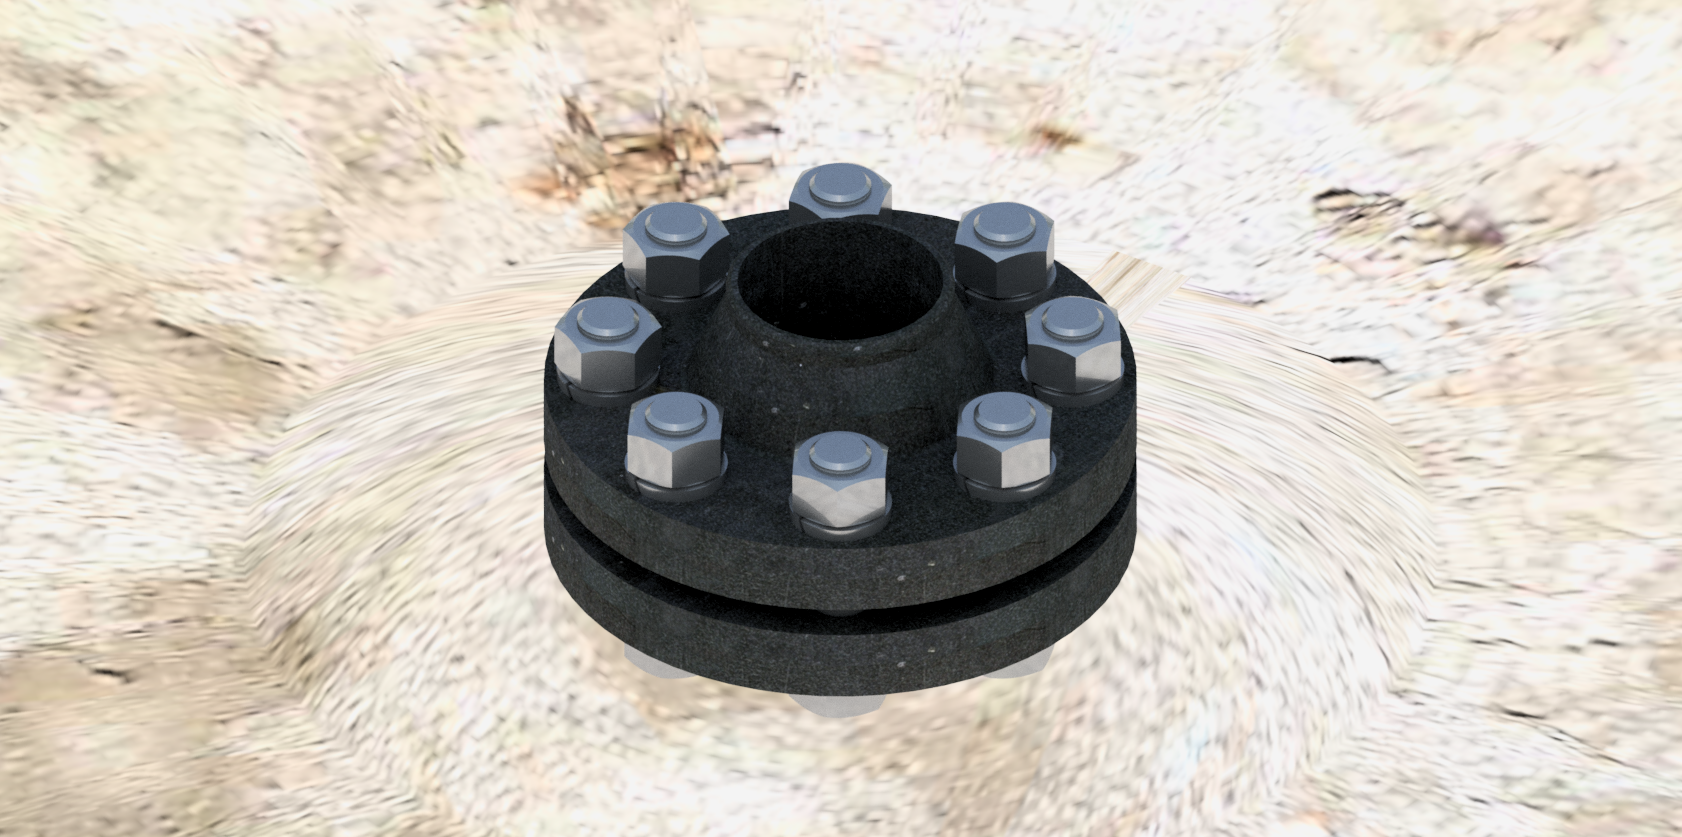
\includegraphics[scale=.34]{./images/assembly.png}
		\caption{Összeállított modell}
	\end{figure}

	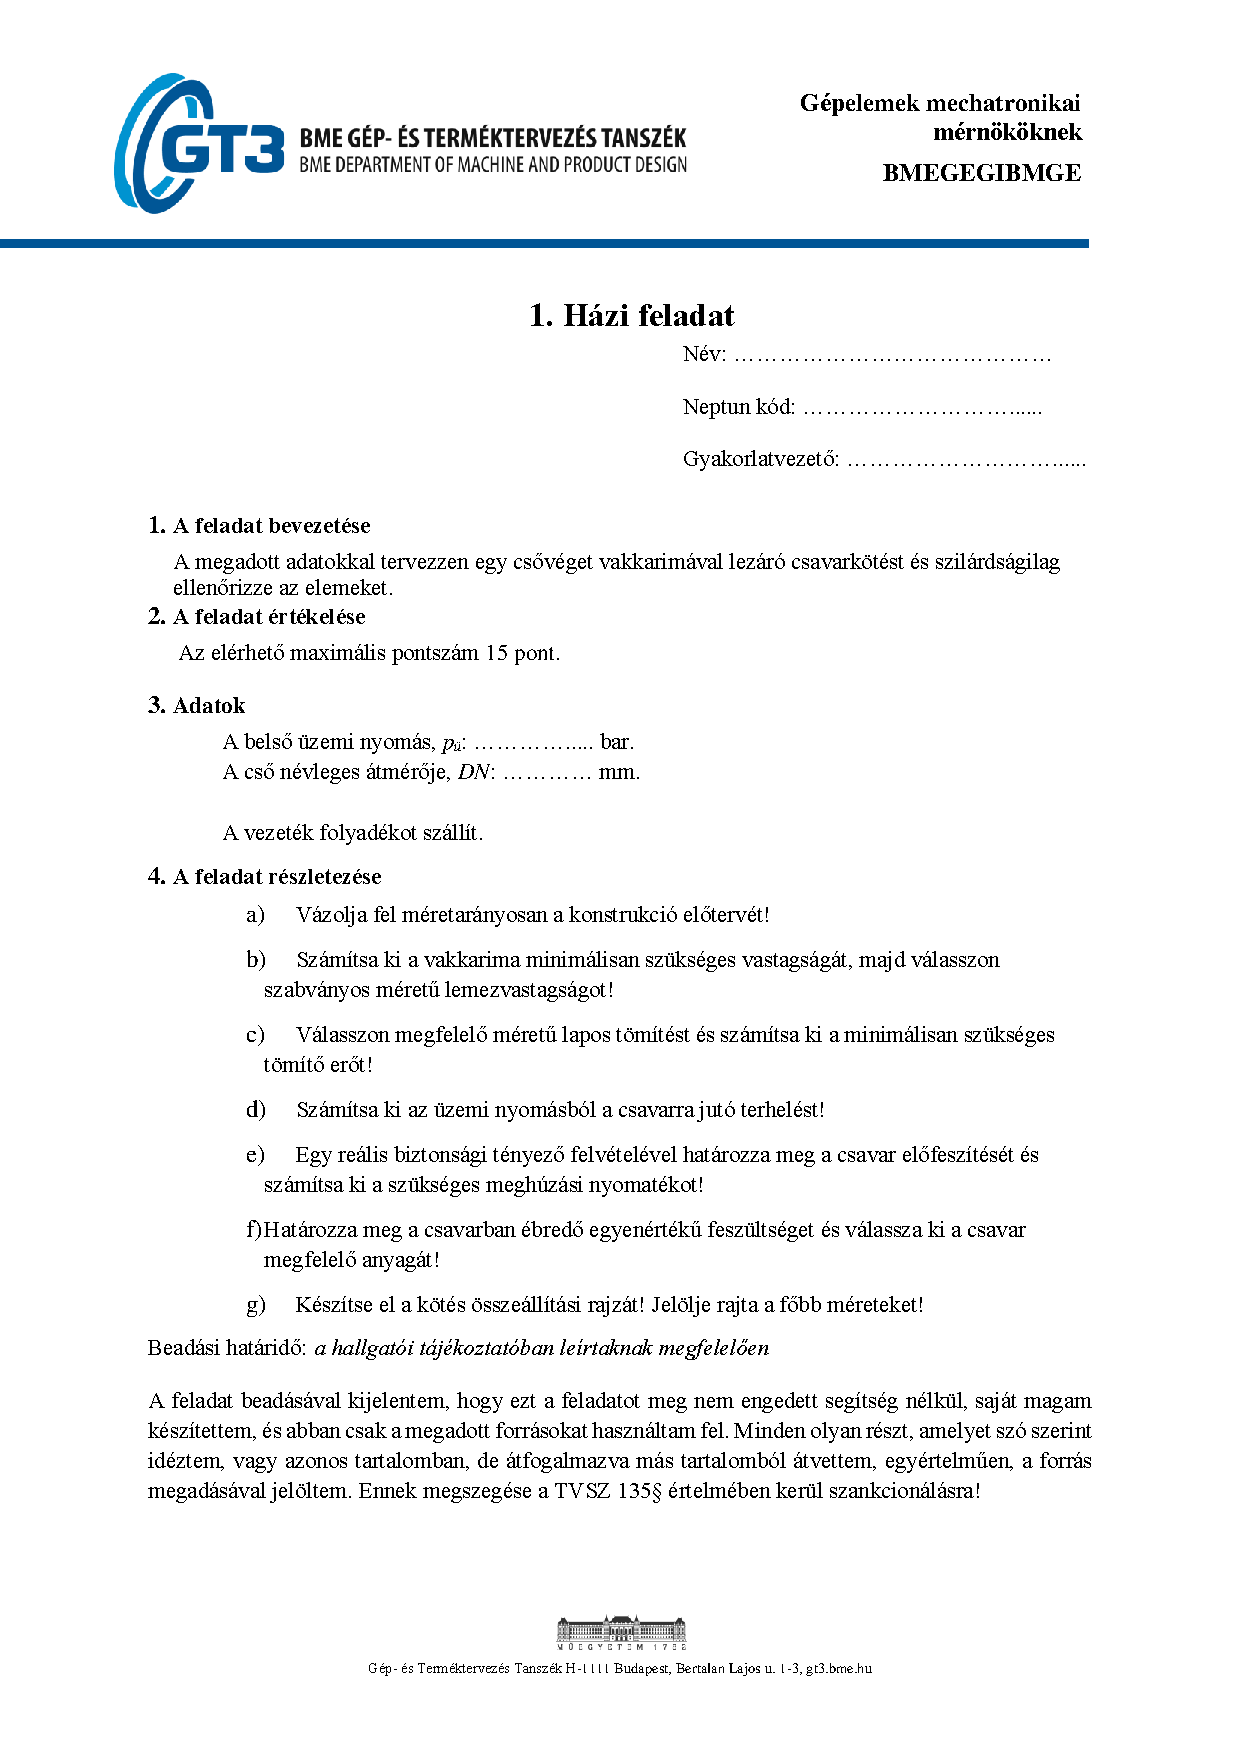
\includepdf[pages={1}, pagecommand={
	\begin{center}
		\begin{picture}(0,0) 
				\put(52, -24.5){Vári Gergő}
				\put(85, -47.5){MQHJ0H}
				\put(104, -72.5){Szabó Gyula}
				\put(-42, -202){\pu}
				\put(-42, -215){\DN}
		\end{picture}
	\end{center}
}]{exercise.pdf}

	
	\tableofcontents

	\newpage
	\pagenumbering{arabic}
	
	\section{Konstrukció előterve}

% TODO

\begin{figure}[hbt!]
	\centering
	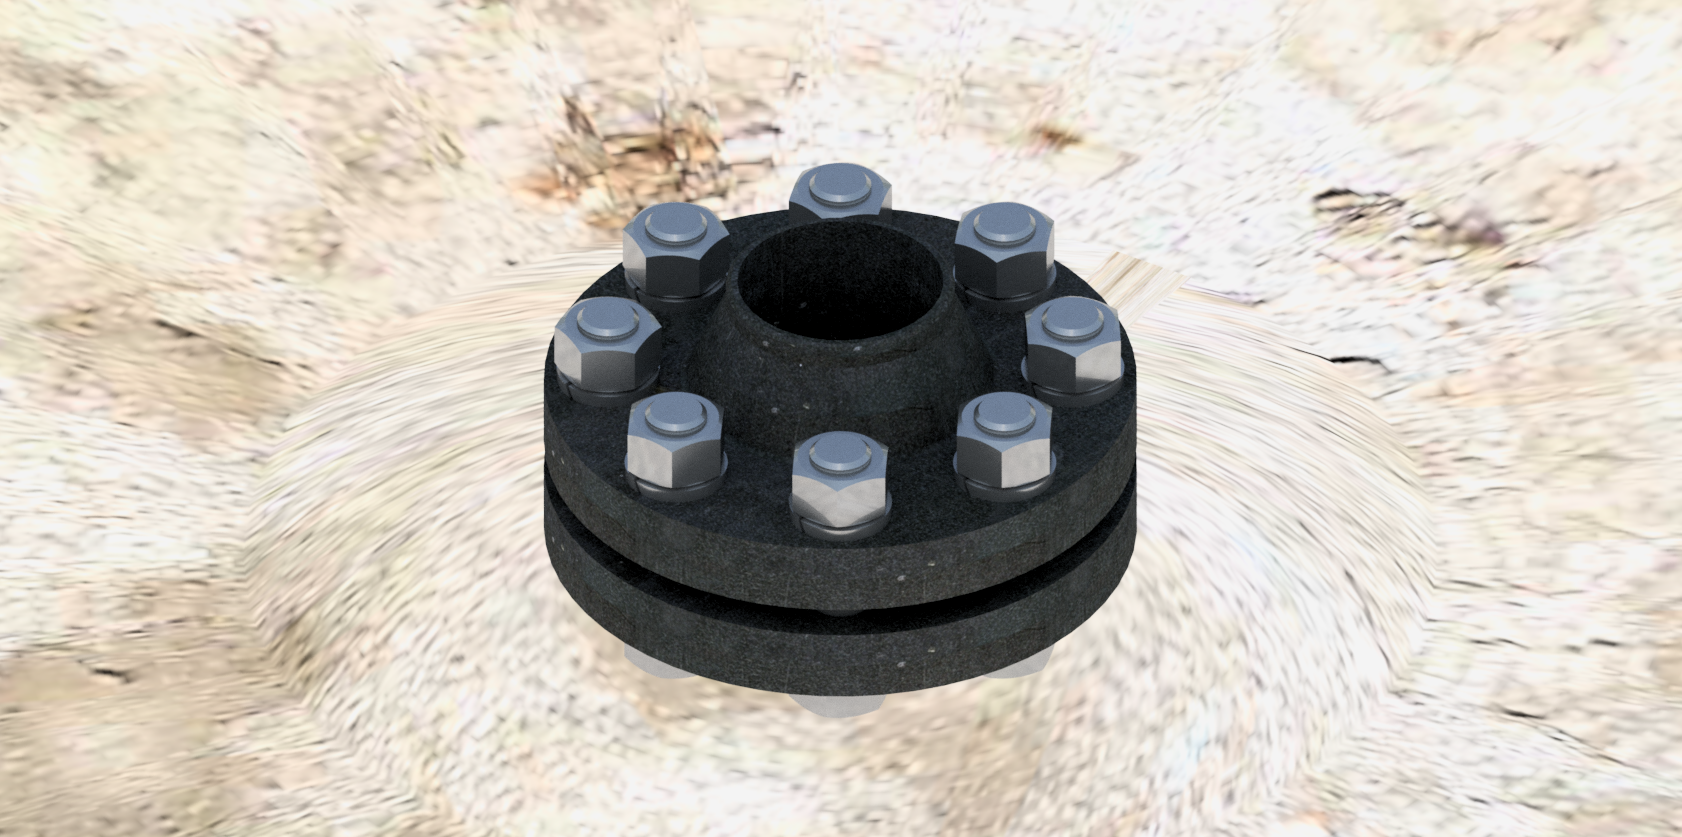
\includegraphics[scale=.1]{./images/assembly.png}
	\caption{Karima előterve}
\end{figure}

	\newpage

	\section{Vakkarima vastagsága és karima szabványok}

\subsection{Szabvány -és anyagválasztás}
% TODO

\newpage
\subsection{Előtervek}
\begin{figure}[hbt!]
	\centering
	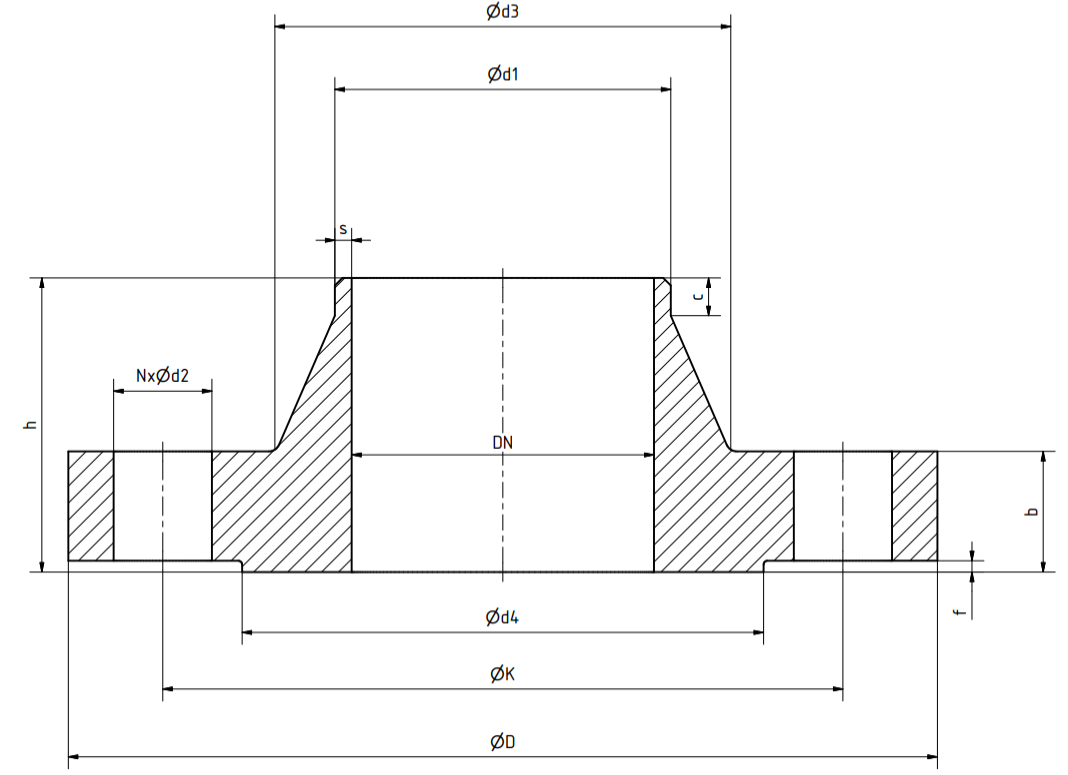
\includegraphics[scale=.61]{./images/karima.png}
	\caption{Karima előtervének rajza}
\end{figure}

\begin{minipage}{.45\linewidth}
	\begin{align*}
		&D = \siunit{\karimaD}{\mm} \\
		&f = \siunit{\karimaf}{\mm} \\
		&d_4 = \siunit{\karimadfour}{\mm} \\
		&d_2 = \siunit{\karimadtwo}{\mm} \\
		&s = \siunit{\karimas}{\mm} \\
		&N = \siunit{\karimaN}{db} \\
		&K = \siunit{\karimaK}{\mm} \\
		&b = \siunit{\karimab}{\mm} \\
		&d_3 = \siunit{\karimadthree}{\mm} \\
		&d_1 = \siunit{\karimadone}{\mm} \\
		&M = \text{M24} \\
		&h = \siunit{\karimah}{\mm}
	\end{align*}
\end{minipage}
\begin{minipage}{.5\linewidth}
	$D$: karima külső átmérő \siunit{}{\mm} \\
	$f$: kiugrás \siunit{}{\mm} \\
	$d_4$: tömítő felület külső átmérő \siunit{}{\mm} \\
	$d_2$: csavar lyukkör \siunit{}{\mm} \\
	$s$: falvastagság \siunit{}{\mm} \\
	$N$: csavarok \siunit{}{db} \\
	$K$: csavarok középátmérő \siunit{}{\mm} \\
	$b$: csavarok alap \\és tömítési sík távolság \siunit{}{\mm} \\
	$d_3$: kúp alsó átmérője \siunit{}{\mm} \\
	$d_1$: cső csatlakozás külső \siunit{}{\mm} \\
	$M$: csavar \siunit{}{\mm} \\
	$h$: karima magasság \siunit{}{\mm}
\end{minipage}

\newpage
\begin{figure}[hbt!]
	\centering
	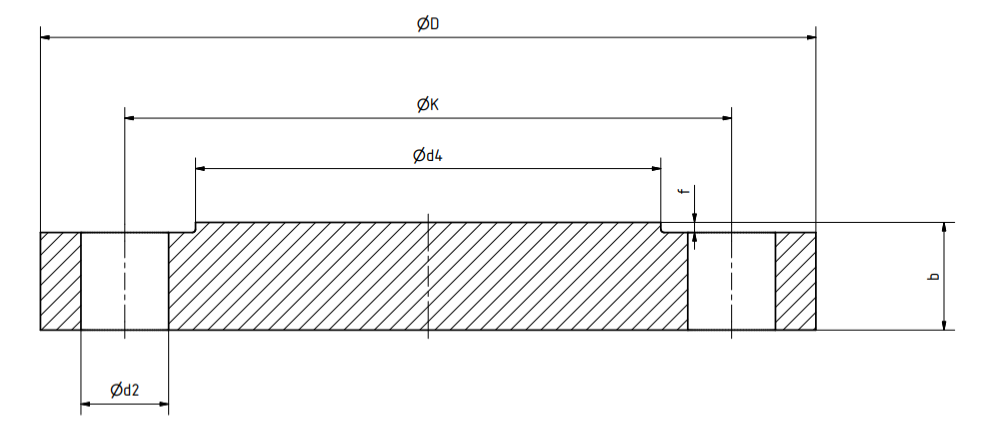
\includegraphics[scale=.34]{./images/vakkarima.png}
	\caption{Vakkarima előtervének rajza}
\end{figure}
\begin{align*}
	&D = \siunit{\karimaD}{\mm} \\
	&f = \siunit{\karimaf}{\mm} \\
	&d_4 = \siunit{\karimadfour}{\mm} \\
	&d_2 = \siunit{\karimadtwo}{\mm} \\
	&K = \siunit{\karimaK}{\mm} \\
	&b = \siunit{\karimab}{\mm} \\
\end{align*}
\begin{center}
	\begin{tabular}{l}
		$D$: vakkarima külső átmérő \siunit{}{\mm} \\
		$f$: kiugrás \siunit{}{\mm} \\
		$d_4$: tömítő felület külső átmérő \siunit{}{\mm} \\
		$d_2$: csavar lyukkör \siunit{}{\mm} \\
		$K$: csavarok középátmérő \siunit{}{\mm} \\
		$b$: vakkarima magassága \siunit{}{\mm} \\
	\end{tabular}
\end{center}

\newpage
\subsection{Minimális vastagság}
\begin{equation}
	d_t = \frac{(d_1 - 2s) + d_4}{2} = \siunit{\karimaDt}{\mm}
\end{equation}

\begin{align}
	&y_k = \frac{k}{\pi} \\
	&y_d = \frac{2}{3} \frac{d_t}{\pi} \\
\end{align}

\begin{equation}
	b_{\text{min}} 
	= \frac{d_t}{2} \sqrt{\frac{3p_\text{ü}}{\sigma_{\text{hajl}}} \left(1-\frac{2}{3} \frac{d_t}{k}\right)} 
	= \siunit{\karimabmin}{\mm}
\end{equation}

\begin{align}
	&\sigma = 
	\frac{d_{t}^2}{4} 
	\frac{3p_{\text{ü}}}{b_{\text{min}}^2}
	\left(1-\frac{2}{3}\frac{d_t}{K}\right) = \mpa{\karimasigma} \\
	&n = \frac{\sigma_{\text{hajl}}}{\sigma} = \siunit{\kariman}{-}
\end{align}

\begin{center}
	\begin{tabular}{l}
		$d_t$: tőmítés középátmérő \siunit{}{\mm} \\
		$d_1$: cső csatlakozás külső \siunit{}{\mm} \\
		$s$: falvastagság \siunit{}{\mm} \\
		$d_4$: tömítő felület külső átmérő \siunit{}{\mm} \\
		$k$: csavar lyukkör \siunit{}{\mm} \\
		$y_k, y_d$: súlypont távolsága a vakkarima kör középpontjától \siunit{}{\mm} \\
		$b_\text{min}$: karima minimális vastagsága \siunit{}{\mm} \\
		$p_\text{ü}$: belső üzemi nyomás \siunit{}{\mm} \\
		$\sigma_\text{hajl}$: maximális hajlító feszültség \siunit{}{\mega\pascal} \\
		$\sigma$: hajlító feszültség minimális karima vastagsággal \siunit{}{\mega\pascal} \\
		$n$: biztonsági tényező \siunit{}{-} \\
	\end{tabular}
\end{center}

	\newpage

	\section{Tömítés kiválasztása}

\subsection{Minimális tömítőerő}

A belső nyomás miatti csőerő hat ellen az üzemi nyomásnak. A gyűrűfelületi csőerő nyom ellen a gyűrű alsó felülete alá benyomódó folyadéknak. A minimális tömítő erő szükséges ahhoz hogy a tömítetség kialakuljon. Ezek összege adja a csavarra ható üzemi erőt.

\begin{align}
	&z = \frac{{d_2}_t - {d_1}_t}{2} = \siunit{\tomz}{db} \\
	&b_t^* = 9 + 0.2z = \siunit{\tombtstar}{\mm}
\end{align}

\begin{align}
	&F_\text{cső} 
	= \frac{\text{DN}^2 \pi}{4} p_\text{ü} = \n{\tomcso} \\
	&F_\text{p} 
	= \frac{\left(d_t^2 - \text{DN}^2\right)\pi}{4} p_\text{ü} 
	= \n{\tomp} \\
	&F_\text{töm} = n_t p_\text{ü} \pi d_t b_t^* = \n{\tomtu}
\end{align}

\begin{equation}
	F_\text{csavar üzemi} 
	= F_\text{cső} + F_\text{p} + F_\text{töm} 
	= \n{\csavaruzemi}
\end{equation}

\begin{align}
	&{n_\text{bizt}}_t = \siunit{\csavarn}{-} \\
	&F_\text{csavar szerelési} 
	= {n_\text{bizt}}_t F_\text{csavar üzemi}
	= \n{\csavarszerel}
\end{align}

\begin{center}
	\begin{tabular}{l}
		$z$: fogak száma \siunit{}{db} \\
		$b_t^*$: tömítés hatásos szélessége \siunit{}{\mm} \\
		$F_\text{cső}$: belső nyomásból származó csőerő \siunit{}{\newton} \\
		$F_\text{p}$: belső nyomásból származó gyűrűfelületi erő \siunit{}{\newton} \\
		$F_\text{töm}$: minimális tömítő erő \siunit{}{\newton} \\
		$F_\text{csavar üzemi}$: csavarokra ható üzemi erő \siunit{}{\newton} \\
		${n_\text{bizt}}_t$: csavarokra ható szerelési erőhöz választott biztonsági tényező \siunit{}{-} \\
		$F_\text{csavar szerelési}$: csavaroknál alkalmazott szerelési erő \siunit{}{\newton} \\
	\end{tabular}
\end{center}

\newpage
\subsection{Szabvány -és anyagválasztás}
A DIN EN 1514-6 B29A PN100 szabvány lett választva  és ez a tömítés nagy nyomásokat is kibír. 1.4541 fémből és egy PTFE borításból készül ahol a fém fésük deformálják a műanyagot az előfeszítés hatására ezzel előidézve a tömítőerőt.

\subsection{Előterv}
\begin{figure}[hbt!]
	\centering
	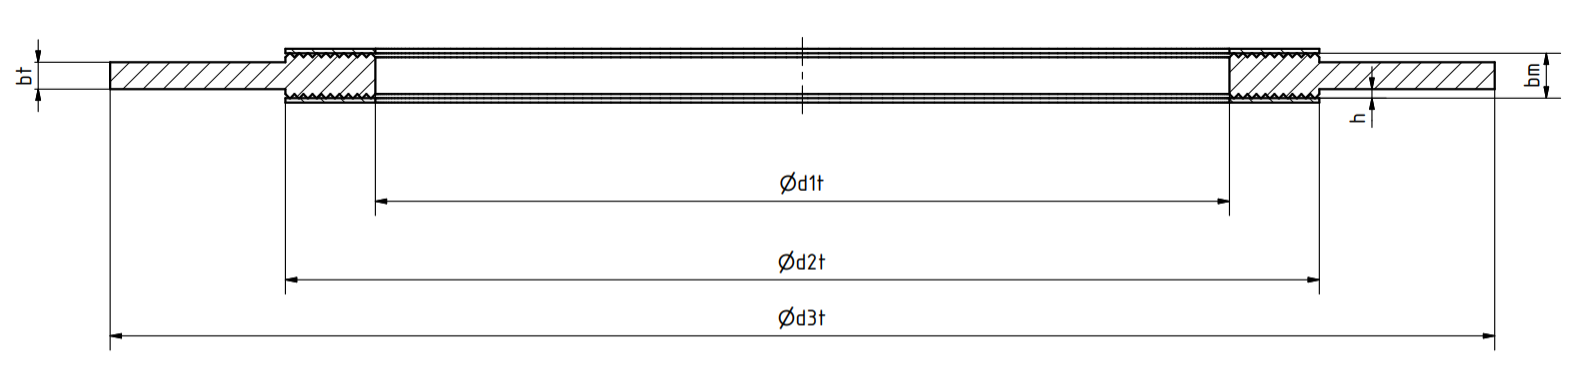
\includegraphics[scale=.34]{./images/tomites.png}
	\caption{Tömítés előtervének rajza}
\end{figure}
\begin{align*}
	&{d_1}_t = \siunit{\tomdone}{\mm} \\
	&{d_2}_t = \siunit{\tomdtwo}{\mm} \\
	&{d_3}_t = \siunit{\tomdthree}{\mm} \\
	&b_t = \siunit{\tombt}{\mm} \\
	&b_m = \siunit{\tombm}{\mm} \\
	&h_{\substack{\text{min}\\\text{max}}} = \substack{\siunit{\tomhmin}{\mm}\\\siunit{\tomhmax}{\mm}} \\
\end{align*}
\begin{center}
	\begin{tabular}{l}
		${d_1}_t$: tőmítés belső átmérő \siunit{}{\mm} \\
		${d_2}_t$: tőmítés felfekvő felület külső átmérő \siunit{}{\mm} \\
		${d_3}_t$: távtartó gyűrű külső átmérő \siunit{}{\mm} \\
		$b_t$: távtartó gyűrű vastagság \siunit{}{\mm} \\
		$b_m$: fém mag magasság \siunit{}{\mm} \\
		$h_{\substack{\text{min}\\\text{max}}}$: szerelés utáni/előtti távolsága \\PTFE lemezeknek a vasmag tetejétől \siunit{}{\mm} \\
	\end{tabular}
\end{center}

	\newpage

	\section[Csavarra jutó terhelés]{Csavarra jutó terhelés\protect\footnote{A feladathoz mellékelt segédletből származó számítások. (9. oldal)}}

A csavar terhelésének kiszámításához a legnagyobb fellépő erő szükséges.

\begin{equation}
	F_v = \frac{F_\text{csavar szerelési}}{n} = \n{\csavarfv}
\end{equation}

\begin{center}
	\begin{tabular}{l}
		$F_v$: csavar terhelése \siunit{}{\newton} \\
		$F_\text{csavar szerelési}$: csavaroknál alkalmazott szerelési erő \siunit{}{\newton} \\
		$n$: csavarok száma \siunit{}{db} \\
	\end{tabular}
\end{center}

	\section{Csavar előfeszítése és meghúzási nyomatéka}

\subsection{Csavar szabvány}
\begin{align*}
	& p = \siunit{\csavarp}{\mm} \\
	& d_3 = \siunit{\csavardthree}{\mm} \\
	& d_2 = \siunit{\csavardtwo}{\mm} \\
	& d_w = \siunit{\csavardw}{\mm} \\
	& b = \siunit{\csavarb}{\mm} \\
	& l = \siunit{\csavarl}{\mm} \\
	& \beta = \siunit{\csavarbeta}{\degree}
\end{align*}

\begin{equation*}
	\mu^{'}_{\substack{\text{min}\\\text{max}}}
	= \substack{
		\siunit{\csavarumin}{-} \\
		\siunit{\csavarumax}{-} \\
	}
\end{equation*}

\subsection{Meghúzási nyomaték}

\begin{align}
	&\mu^{'}_{\substack{\text{min}\\\text{max}}}
	= \frac
		{\mu_{\substack{\text{min}\\\text{max}}}}
		{\cos{\frac{\beta}{2}}} \\
	&\rho^{'}_{\substack{\text{min}\\\text{max}}} 
	= \arctan{\mu^{'}_{\substack{\text{min}\\\text{max}}}}
	= \substack{
		\siunit{\csavarptmin}{\degree} \\
		\siunit{\csavarptmax}{\degree}
	}
\end{align}

\begin{align}
	&{M_\text{csavar}}_{\substack{\text{min}\\\text{max}}} 
	= F_v \frac{{d_2}_\text{cs}}{2} \tan{\left(\alpha + {\rho^{'}}_{\substack{\text{min}\\\text{max}}}\right)} 
	= \substack{
		\siunit{\csavarMcsmin}{\newton\mm} \\
		\siunit{\csavarMcsmax}{\newton\mm}
	}\\
	&{M_\text{anya}}_{\substack{\text{min}\\\text{max}}} 
	= F_v \frac{d_a}{2} {\mu^{'}_{\substack{\text{min}\\\text{max}}}}  
	= \substack{
		\siunit{\csavarMamin}{\newton\mm} \\
		\siunit{\csavarMamax}{\newton\mm}
	}\\
\end{align}

\begin{equation}
	{M_\text{meghúzási}}_{\substack{\text{min}\\\text{max}}} = {M_\text{csavar}}_{\substack{\text{min}\\\text{max}}} + {M_\text{anya}}_{\substack{\text{min}\\\text{max}}}
	= \substack{
		\siunit{\csavarmegmin}{\newton\mm} \\
		\siunit{\csavarmegmax}{\newton\mm}
	}\\
\end{equation}

	\newpage

	\section{Csavar anyagválasztás}

\subsection{Redukált feszültség}

A legnagyobb igénybevételre ($\sigma_\text{red}$) kell méretezni és ez a húzó ($\sigma$) illetve csavaró ($\tau$) nyomaték összege.

\begin{align}
	&A_e = \frac{\left({\frac{{d_2}_\text{cs} + {d_3}_\text{cs}}{2}}\right)^2 \pi}{4} = \siunit{\csavarae}{\mm^2} \\
	&\sigma = \frac{F_v}{A_e} = \siunit{\csavarsigma}{\mega\pascal}
\end{align}

\begin{align}
	&K_p = \frac{\left(\frac{{d_2}_\text{cs} + {d_3}_\text{cs}}{2}\right)^3 \pi}{16} = \siunit{\csavarkp}{\mm^3} \\
	&M_\text{csavar} = {M_\text{anya}}_\text{max} \\
	&\tau = \frac{M_\text{csavar}}{K_p} = \mpa{\csavartau}
\end{align}

\begin{equation}
	\sigma_\text{red} = \sqrt{\sigma^2 + 3\tau^2} = \mpa{\csavarred}
\end{equation}

\subsection{Méretezés}

A kiszámolt feszültséggel már lehet szilárdsági osztályt választani és a 3.6-os megfelel az igényeknek (hiszen $R_\text{eH}$ nagyobb az elvártnál).

\begin{align}
	&R_\text{eH} = \mpa{\csavarreh} \\
	&{n_\text{bizt}}_\text{cs} = \frac{R_\text{eh}}{\sigma_\text{red}} = \siunit{\csavarntwo}{-}
\end{align}

\begin{center}
	\begin{tabular}{l}
		$A_e$: csavarerőt vivő keresztmetszet terület \siunit{}{\mm^2} \\
		${d_2}_\text{cs}$: menet középátmérő \siunit{}{\mm} \\
		${d_3}_\text{cs}$: orsó magátmérő \siunit{}{\mm} \\
		$\sigma$: húzó feszültség \siunit{}{\mega\pascal} \\
		$F_v$: csavar terhelése \siunit{}{\newton} \\
		$K_p$: csavar keresztmetszet poláris másodrendű nyomaték \siunit{}{\mm^3} \\
		$M_\text{csavar}$: csavar mentén súrlódásból származó csavaró nyomaték \siunit{}{\newton\mm} \\
		${M_\text{anya}}_{\text{max}}$: csavaranya felülete alatti maximum súrlódás \siunit{}{\newton\mm} \\
		$\tau$: csavaró feszültség \siunit{}{\mega\pascal} \\
		$\sigma_\text{red}$: redukált feszültség \siunit{}{\mega\pascal} \\
		$R_\text{eH}$: folyáshatár \siunit{}{\mega\pascal} \\
		${N_\text{bizt}}_\text{cs}$: csavar biztonsági tényező \siunit{}{-} \\
	\end{tabular}
\end{center}

	\newpage
	
	\stepcounter{section}
\addtocontents{toc}{\protect\contentsline{section}{\protect\numberline{\thesection}Összeállítási rajz}{}{}}

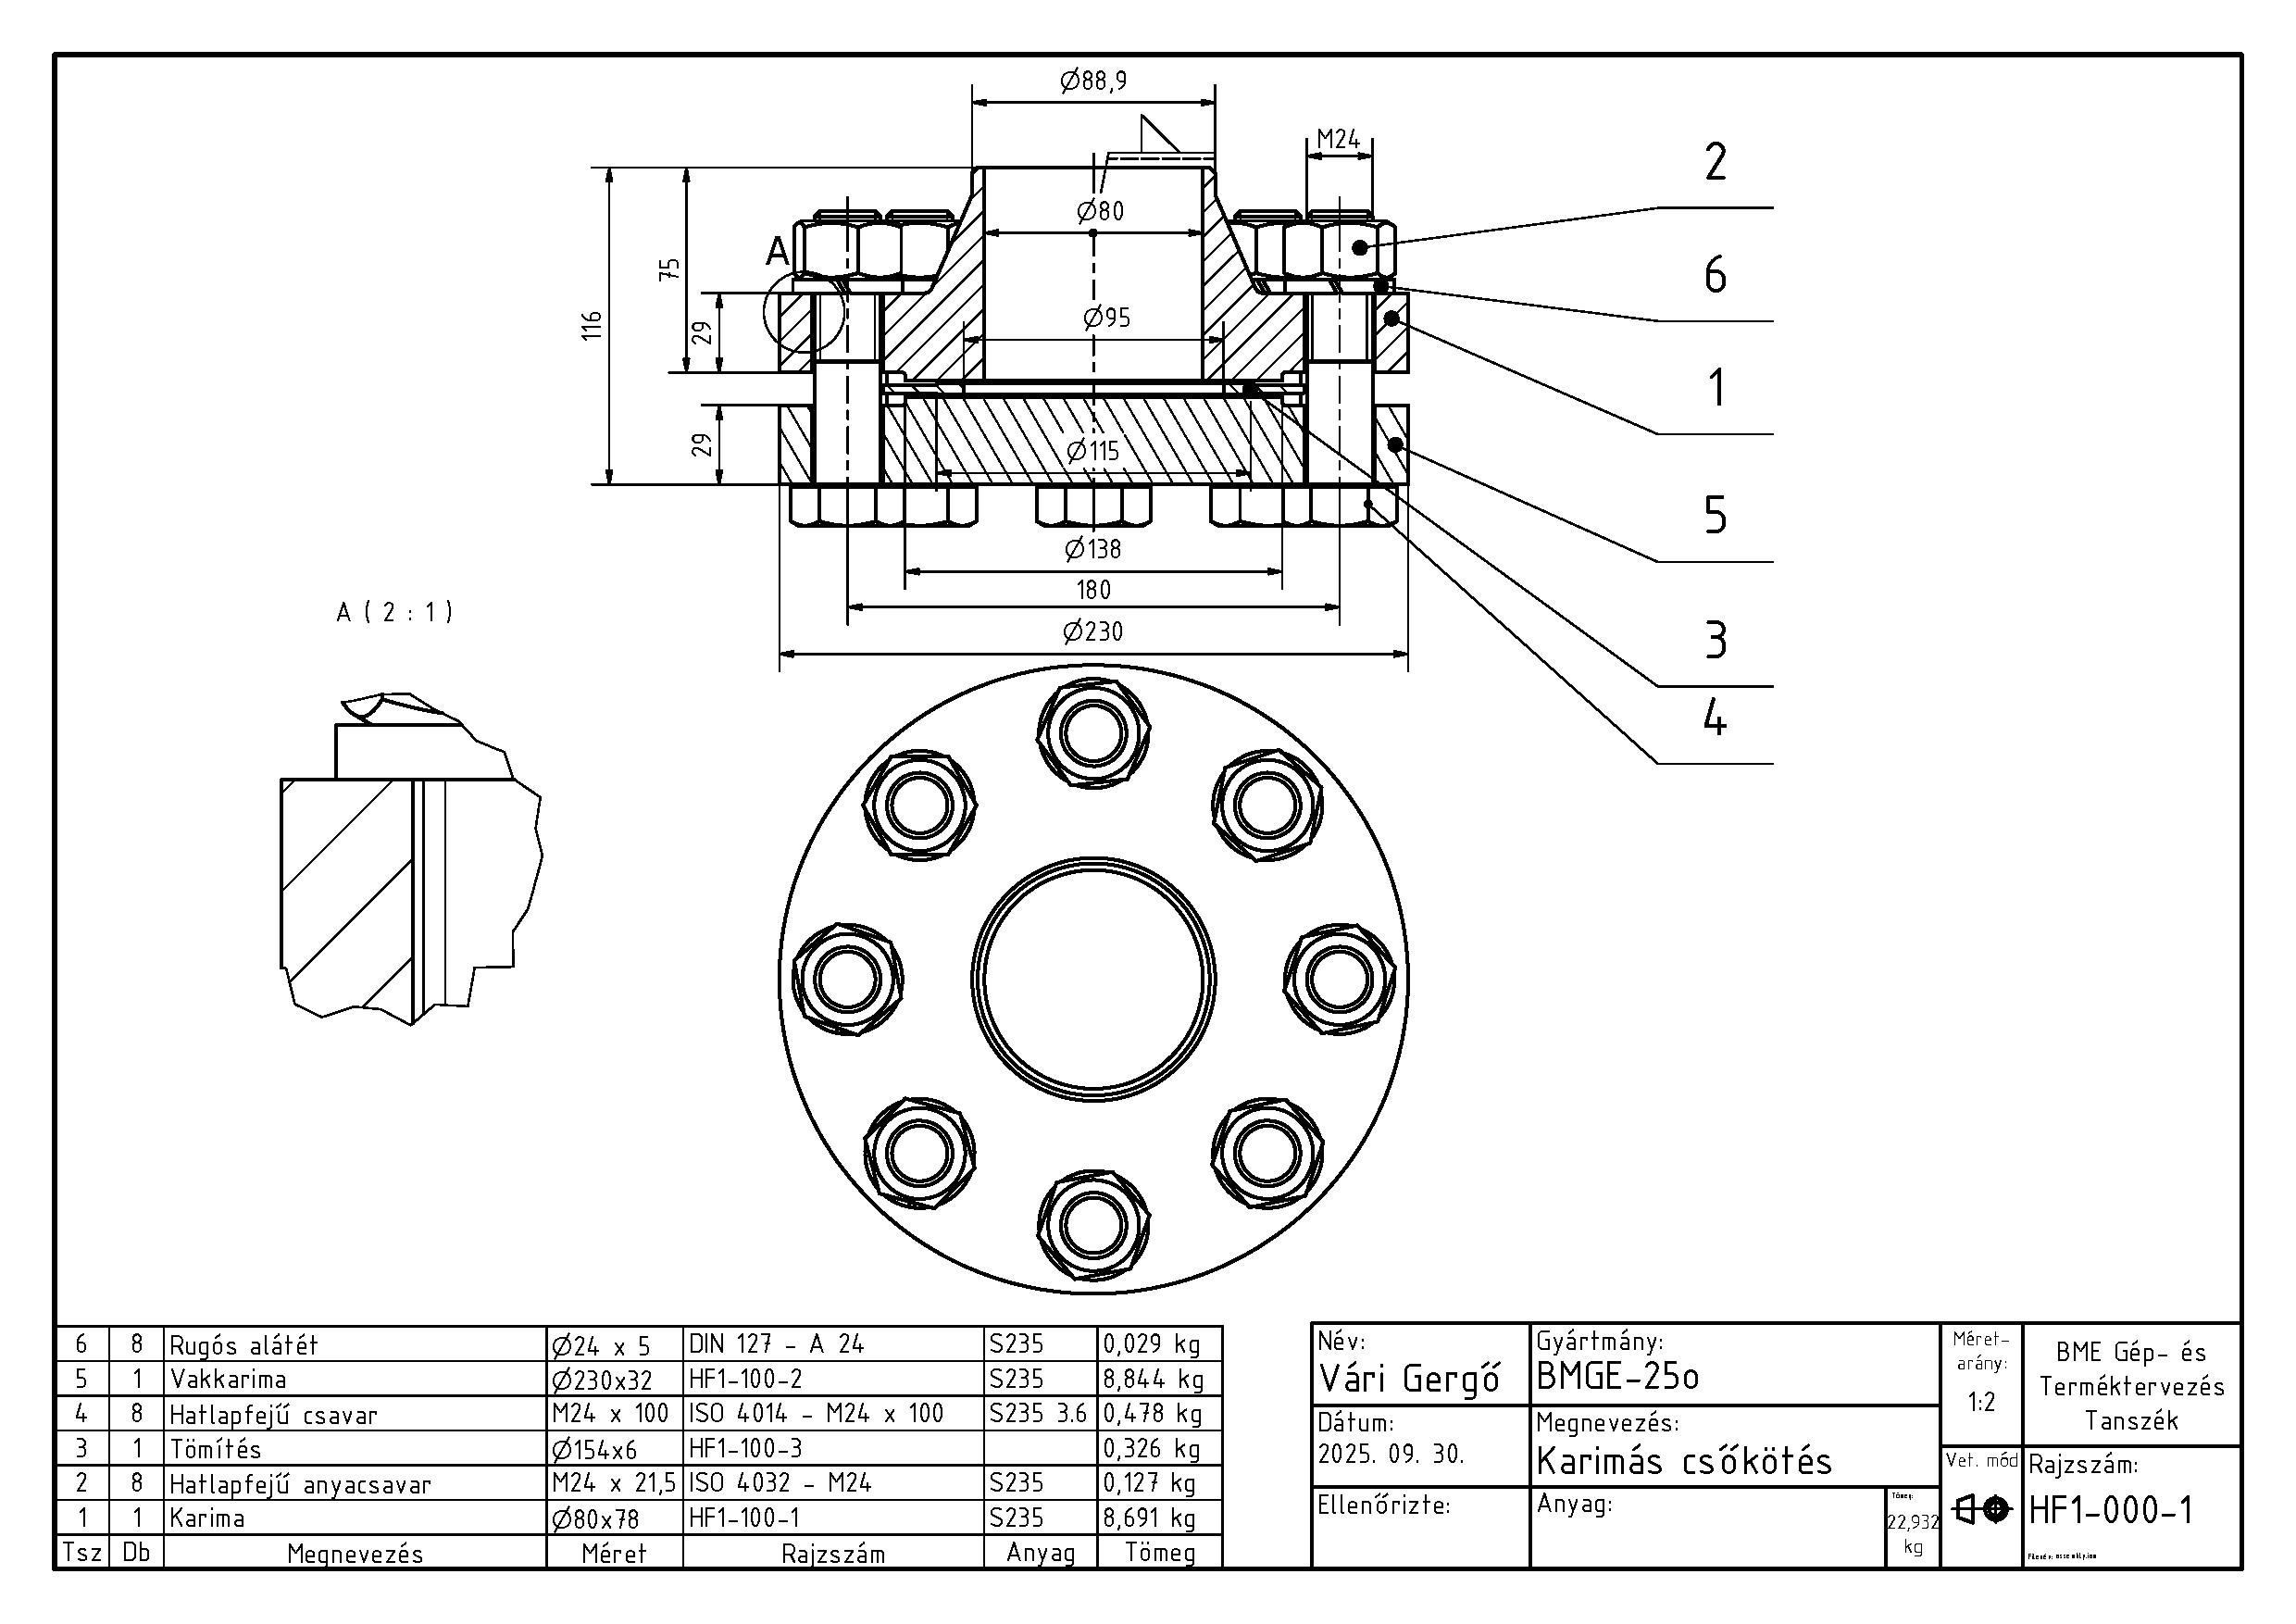
\includepdf{assembly.pdf}

\end{document}
